\makesectionpage[figures/quiz.png]{Schwarmintelligenz}

\begin{frame}{Schwarmintelligenz: Grundidee}
\begin{columns}
\begin{column}{0.35\textwidth}
  \
\centering

\end{column}

\begin{column}{0.60\textwidth}
\textbf{Schwarmintelligenz} bezeichnet kollektives, scheinbar intelligentes Verhalten, das aus dem Zusammenwirken vieler einfacher Individuen entsteht.

\vspace{0.5em}
\begin{itemize}
\item Kein Individuum besitzt einen \textbf{Gesamtplan}.
\item Jedes folgt nur \textbf{einfachen, lokalen Regeln}.
\item Aus lokaler Interaktion entsteht globale Ordnung (\textbf{Emergenz}).
\end{itemize}
\end{column}
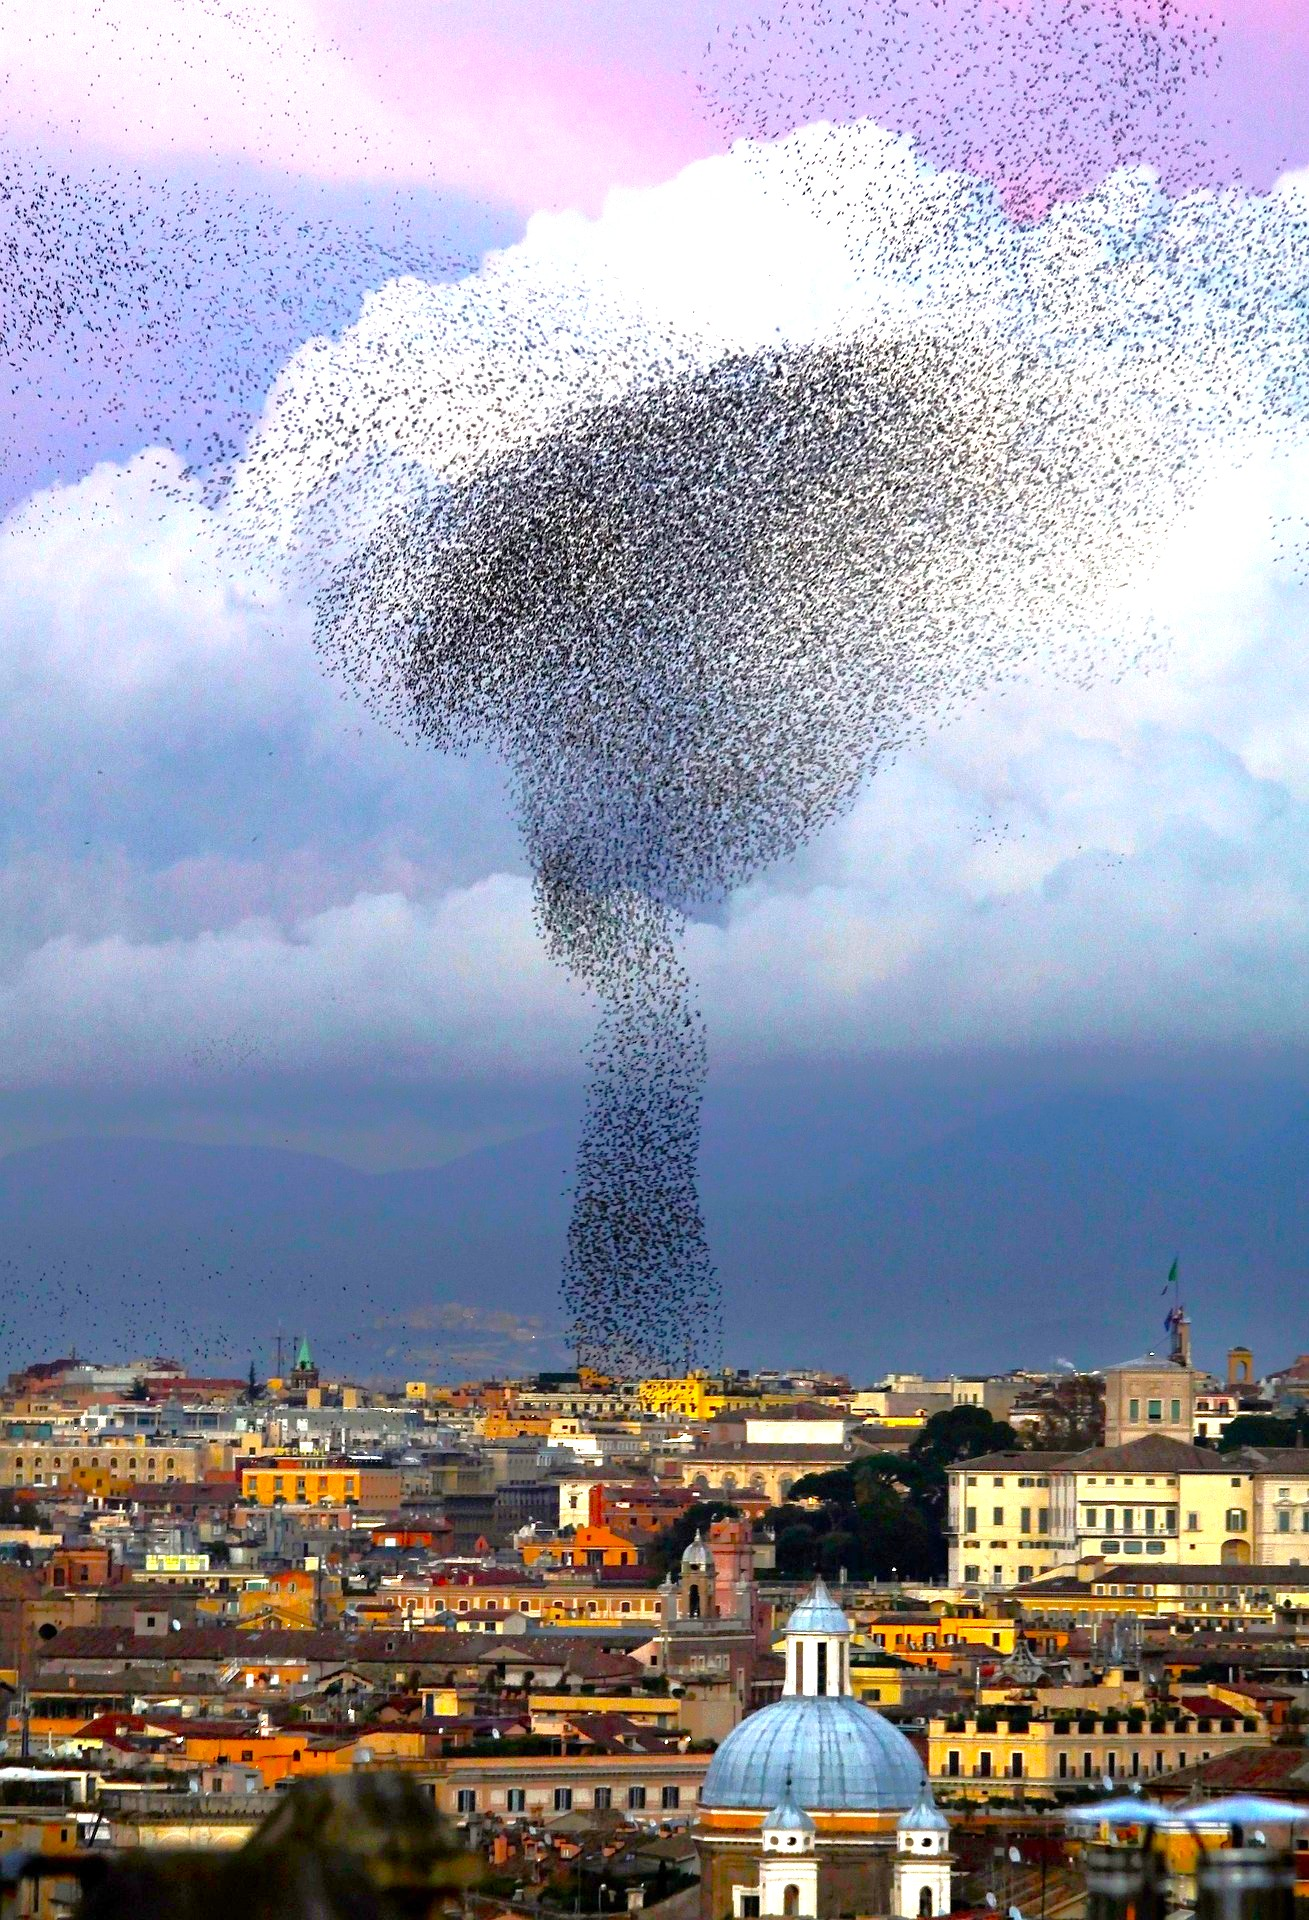
\includegraphics[width=\linewidth]{figures/vogelschwarm.jpg}
\end{columns}
\end{frame}

\begin{frame}{Schwarmintelligenz in der Natur}
\begin{columns}
\begin{column}{0.70\textwidth}
Viele biologische Systeme lösen komplexe Aufgaben ohne zentrale Steuerung:
\begin{itemize}
\item \textbf{Ameisen} finden über Pheromonspuren kürzeste Wege.
\item \textbf{Vögel} bilden stabile Schwärme ohne Anführer.
\item \textbf{Fische} weichen Räubern koordiniert aus.
\item \textbf{Bienen} entscheiden gemeinsam über neue Nistplätze.
\end{itemize}
\end{column}
\begin{column}{0.25\textwidth}
\centering
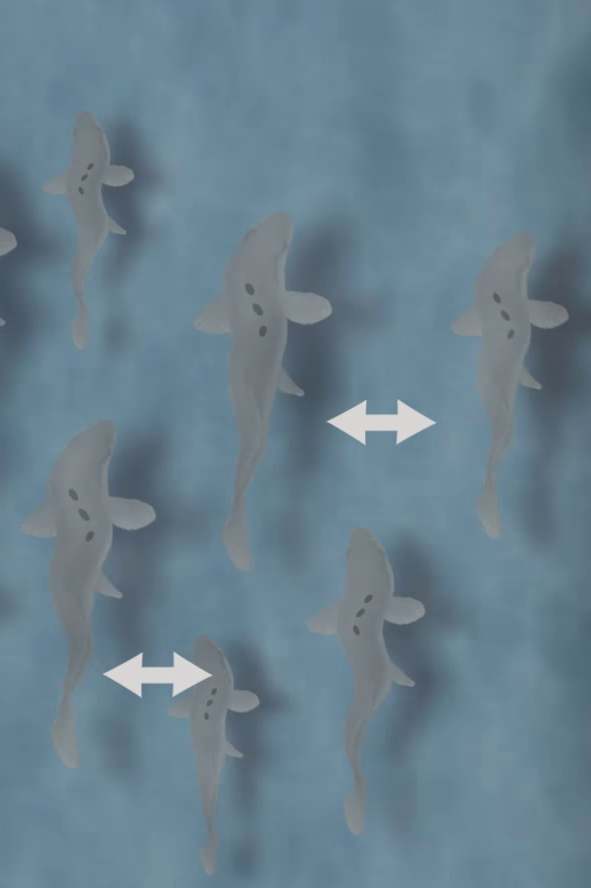
\includegraphics[width=\linewidth]{figures/video_schwarm_stichlinge.png}
\footnotesize Video: ,,Gut zu wissen: Warum stoßen Fische im Schwarm nie zusammen?''
\end{column}
\end{columns}
\source{\cite{tagesschau2021video121}}
\end{frame}

\begin{frame}{Prinzipien des Schwarmverhaltens}
\begin{columns}
\begin{column}{0.60\textwidth}
Reynolds beschrieb 1987 das Verhalten von Schwärmen (\textbf{Boids}) durch drei Regeln:
\begin{itemize}
\item \textbf{Separation}: Abstand zu Nachbarn halten.
\item \textbf{Alignment}: Richtung an Nachbarn angleichen.
\item \textbf{Kohäsion}: zum Mittelpunkt der Nachbarn streben.
\end{itemize}
Diese lokalen Regeln erzeugen das koordinierte Gesamtbild.
\end{column}
\begin{column}{0.35\textwidth}
\resizebox{\linewidth}{!}{%
\begin{tikzpicture}[>=stealth, every node/.style={font=\scriptsize}]
\foreach \x/\y in {0/0, 0.7/0.4, 1.4/0.1, 0.5/1.0, 1.3/1.1, 0.2/1.7} {
  \draw[->, AccentColor, very thick] (\x,\y) -- ++(0.7,0.3);
}
\node at (0.9,-0.7) {gemeinsame Richtung};
\end{tikzpicture}%
}
\end{column}
\end{columns}
\end{frame}

\begin{frame}{Eigenschaften intelligenter Schwärme}
\begin{columns}
\begin{column}{0.60\textwidth}
Schwarmsysteme zeigen typische Merkmale:
\begin{itemize}
\item \textbf{Dezentralisierung}: keine zentrale Kontrolle.
\item \textbf{Selbstorganisation}: Struktur entsteht von selbst.
\item \textbf{Robustheit}: Ausfall Einzelner ist unkritisch.
\item \textbf{Skalierbarkeit}: funktioniert für kleine und große Populationen.
\end{itemize}
\end{column}
\begin{column}{0.35\textwidth}
Das Verhalten des Kollektivs ist \textbf{mehr} als die Summe der Einzelverhalten.
\end{column}
\end{columns}
\end{frame}

\begin{frame}{Von der Natur zur Optimierung}
\begin{columns}
\begin{column}{0.60\textwidth}
Die Grundidee lässt sich auf \textbf{Optimierungsprobleme} übertragen:
\begin{itemize}
\item Individuen werden zu \textbf{Suchpunkten} im Lösungsraum.
\item Ihre Bewegung wird durch \textbf{eigene} und \textbf{gemeinsame} Erfahrung gelenkt.
\item Der Schwarm konvergiert gemeinsam zu guten Lösungen.
\end{itemize}
Dieses Prinzip führt zur \textbf{Partikelschwarmoptimierung}.
\end{column}
\begin{column}{0.35\textwidth}
\centering
\twemoji[width=0.9\linewidth]{bird}
\end{column}
\end{columns}
\end{frame}

\begin{frame}{Partikelschwarmoptimierung: Überblick}
\begin{columns}
\begin{column}{0.60\textwidth}
Die \textbf{Partikelschwarmoptimierung} (PSO) wurde 1995 von \textbf{Kennedy} und \textbf{Eberhart} vorgestellt.

\vspace{0.5em}
\begin{itemize}
\item Ein \textbf{Schwarm} aus Partikeln durchsucht den Lösungsraum.
\item Jedes Partikel ist eine \textbf{Kandidatenlösung}.
\item Partikel orientieren sich am \textbf{eigenen} und am \textbf{besten} bekannten Ergebnis.
\end{itemize}
PSO ist ein \textbf{populationsbasiertes}, ableitungsfreies Verfahren.
\end{column}
\begin{column}{0.35\textwidth}
Geeignet für nichtlineare, nicht differenzierbare und hochdimensionale Probleme.
\end{column}
\end{columns}
\source{\cite{kennedy1995particle}}
\end{frame}

\begin{frame}{Das Optimierungsproblem}
\begin{columns}
\begin{column}{0.60\textwidth}
Gesucht wird das Minimum einer \textbf{Zielfunktion}:
\[
\min_{x \in \mathbb{R}^n} f(x)
\]
\begin{itemize}
\item $x$ ist ein Punkt im $n$-dimensionalen \textbf{Suchraum}.
\item $f(x)$ bewertet die \textbf{Güte} einer Lösung (Fitness).
\item Ein Maximierungsproblem entspricht dem Minimieren von $-f(x)$.
\end{itemize}
\end{column}
\begin{column}{0.35\textwidth}
Die Funktion $f$ muss \textbf{nur auswertbar} sein, nicht differenzierbar.
\end{column}
\end{columns}
\source{\cite{kennedy1995particle}}
\end{frame}

\begin{frame}{Ein Partikel}
\begin{columns}
\begin{column}{0.60\textwidth}
Jedes Partikel $i$ besitzt:
\begin{itemize}
\item eine \textbf{Position} $x_i$ (aktuelle Lösung),
\item eine \textbf{Geschwindigkeit} $v_i$ (Bewegungsrichtung),
\item sein \textbf{persönliches Bestes} $p_i$ (beste bisher besuchte Position).
\end{itemize}
In jedem Schritt bewegt sich das Partikel gemäß seiner Geschwindigkeit weiter.
\end{column}
\begin{column}{0.35\textwidth}
\resizebox{\linewidth}{!}{%
\begin{tikzpicture}[>=stealth, every node/.style={font=\scriptsize}]
\node[circle,fill=PrimaryColor,inner sep=2pt,label=below:{$x_i$}] (x) at (0,0) {};
\node[circle,fill=AccentColor,inner sep=2pt,label=above:{$p_i$}] (p) at (2.2,1.6) {};
\draw[->,PrimaryTitle,very thick] (x) -- ++(1.4,0.5) node[midway,below] {$v_i$};
\draw[dashed,gray] (x) -- (p);
\end{tikzpicture}%
}
\end{column}
\end{columns}
\source{\cite{kennedy1995particle}}
\end{frame}

\begin{frame}{Persönliches und globales Bestes}
\begin{columns}
\begin{column}{0.60\textwidth}
Der Schwarm nutzt zwei Gedächtnisse:
\begin{itemize}
\item $p_i$ (\textbf{pbest}): beste Position, die Partikel $i$ selbst gefunden hat.
\item $g$ (\textbf{gbest}): beste Position, die \textbf{der gesamte Schwarm} gefunden hat.
\end{itemize}

\vspace{0.5em}
Das globale Beste wird laufend aktualisiert:
\[
g = \arg\min_{i} f(p_i)
\]
\end{column}
\begin{column}{0.35\textwidth}
$p_i$ steht für \textbf{eigene Erfahrung}, $g$ für \textbf{soziales Wissen} des Schwarms.
\end{column}
\end{columns}
\source{\cite{kennedy1995particle}}
\end{frame}

\begin{frame}{Geschwindigkeitsupdate}
\begin{columns}
\begin{column}{0.47\textwidth}
Die neue Geschwindigkeit setzt sich aus drei Anteilen zusammen:
\[
v_i^{t+1} = \textcolor{PrimaryColor}{v_i^{t}}
+ \textcolor{AccentColor}{c_1 r_1 (p_i - x_i^{t})}
+ \textcolor{AlertColor}{c_2 r_2 (g - x_i^{t})}
\]
\begin{itemize}
\item \textcolor{PrimaryColor}{\textbf{Trägheit}}: bisherige Richtung.
\item \textcolor{AccentColor}{\textbf{kognitiv}}: Zug zum eigenen Besten.
\item \textcolor{AlertColor}{\textbf{sozial}}: Zug zum globalen Besten.
\end{itemize}
\end{column}
\begin{column}{0.48\textwidth}
\resizebox{\linewidth}{!}{%
\begin{tikzpicture}[>=stealth, every node/.style={font=\scriptsize}]
\coordinate (xi) at (0,0);
\coordinate (pi) at (4,2.6);
\coordinate (g)  at (5,-0.6);
\coordinate (A)  at (1.3,0.35);
\coordinate (B)  at (2.4,1.0);
\coordinate (C)  at (3.6,0.75);
\node[circle,fill=PrimaryColor,inner sep=1.5pt,label=below left:{$x_i^{t}$}] at (xi) {};
\node[circle,fill=AccentColor,inner sep=1.5pt,label=above:{$p_i$}] at (pi) {};
\node[circle,fill=AlertColor,inner sep=1.5pt,label=below:{$g$}] at (g) {};
\node[circle,fill=PrimaryTitle,inner sep=1.5pt,label=above right:{$x_i^{t+1}$}] at (C) {};
\draw[dashed,gray] (xi) -- (pi);
\draw[dashed,gray] (xi) -- (g);
\draw[->,PrimaryColor,very thick] (xi) -- (A);
\draw[->,AccentColor,very thick] (A) -- (B);
\draw[->,AlertColor,very thick] (B) -- (C);
\draw[->,PrimaryTitle,ultra thick] (xi) -- (C) node[midway,below right] {$v_i^{t+1}$};
\end{tikzpicture}%
}
\end{column}
\end{columns}
\source{\cite{kennedy1995particle}}
\end{frame}

\begin{frame}{Positionsupdate}
\begin{columns}
\begin{column}{0.60\textwidth}
Nach der Geschwindigkeit wird die \textbf{Position} aktualisiert:
\[
x_i^{t+1} = x_i^{t} + v_i^{t+1}
\]
\begin{itemize}
\item Das Partikel bewegt sich entlang der neuen Geschwindigkeit.
\item Anschließend wird $f(x_i^{t+1})$ bewertet.
\item Bei Verbesserung werden $p_i$ und ggf. $g$ aktualisiert.
\end{itemize}
\end{column}
\begin{column}{0.35\textwidth}
Geschwindigkeit und Position werden für \textbf{jedes} Partikel in jedem Schritt neu berechnet.
\end{column}
\end{columns}
\source{\cite{kennedy1995particle}}
\end{frame}

\begin{frame}{Die Parameter}
\begin{columns}
\begin{column}{0.47\textwidth}
\begin{itemize}
\item $c_1$: \textbf{kognitiver} Faktor (Vertrauen in sich selbst).
\item $c_2$: \textbf{sozialer} Faktor (Vertrauen in den Schwarm).
\item $r_1, r_2 \in [0,1]$: \textbf{Zufallswerte} pro Schritt.
\item $w$: \textbf{Trägheitsgewicht} (spätere Erweiterung).
\end{itemize}
\end{column}
\begin{column}{0.48\textwidth}
\begin{itemize}
\item Großes $c_1$: starke \textbf{Exploration}.
\item Großes $c_2$: schnelle \textbf{Konvergenz}.
\item Die Zufallswerte sorgen für \textbf{Vielfalt} im Schwarm.
\end{itemize}
Typisch: $c_1 \approx c_2 \approx 2$.
\end{column}
\end{columns}
\source{\cite{kennedy1995particle}}
\end{frame}

\begin{frame}{Der PSO-Algorithmus}
\begin{columns}
\begin{column}{0.60\textwidth}
\footnotesize
\begin{algorithm}[H]
\DontPrintSemicolon
\SetKwInOut{Input}{Input}
\SetKwInOut{Output}{Output}
\Input{Zielfunktion $f$, Schwarmgröße $N$, $c_1$, $c_2$}
\Output{beste Position $g$}
\ForEach{Partikel $i \in \{1,\dots,N\}$}{
  Initialisiere $x_i$ und $v_i$ zufällig\;
  $p_i \leftarrow x_i$\;
}
$g \leftarrow \arg\min_i f(p_i)$\;
\Repeat{Abbruchkriterium erfüllt}{
  \ForEach{Partikel $i$}{
    $r_1, r_2 \leftarrow$ Zufall in $[0,1]$\;
    $v_i \leftarrow v_i + c_1 r_1 (p_i - x_i) + c_2 r_2 (g - x_i)$\;
    $x_i \leftarrow x_i + v_i$\;
    \If{$f(x_i) < f(p_i)$}{
      $p_i \leftarrow x_i$\;
    }
    \If{$f(p_i) < f(g)$}{
      $g \leftarrow p_i$\;
    }
  }
}
\end{algorithm}
\end{column}
\begin{column}{0.35\textwidth}
Der Schwarm wiederholt \textbf{Bewegung} und \textbf{Bewertung}, bis er konvergiert oder eine Schranke erreicht ist.
\end{column}
\end{columns}
\source{\cite{kennedy1995particle}}
\end{frame}

\begin{frame}{Ablauf: Konvergenz des Schwarms}
\begin{columns}
\begin{column}{0.35\textwidth}
\resizebox{\linewidth}{!}{%
\begin{tikzpicture}[>=stealth, every node/.style={font=\scriptsize}]
\node[star,star points=5,fill=AlertColor,draw=AlertColor,
      minimum size=0.6cm,inner sep=0pt,label=below:{$g$}] (opt) at (0,0) {};
\foreach \x/\y in {-3/1.5, -2.5/-1.2, 2.8/1.0, 3.2/-0.8,
                   -1.5/2.2, 1.8/-2.0, 0.3/2.6, -3.2/-0.3} {
  \node[circle,fill=PrimaryColor,inner sep=1.5pt] at (\x,\y) {};
  \draw[->,AccentColor,thick] (\x,\y) -- ($ (\x,\y)!0.45!(0,0) $);
}
\end{tikzpicture}%
}
\end{column}
\begin{column}{0.60\textwidth}
Während des Laufs bewegt sich der Schwarm gemeinsam auf gute Regionen zu:
\begin{itemize}
\item Anfangs sind die Partikel \textbf{breit gestreut} (Exploration).
\item Über die Zeit ziehen sie zum \textbf{globalen Besten} (Exploitation).
\item Schließlich \textbf{konzentriert} sich der Schwarm um das Optimum.
\end{itemize}
\end{column}
\end{columns}
\source{\cite{kennedy1995particle}}
\end{frame}

\begin{frame}{Erweiterungen des Grundverfahrens}
\begin{columns}
\begin{column}{0.60\textwidth}
Das Grundmodell wurde vielfach verbessert:
\begin{itemize}
\item \textbf{Trägheitsgewicht} $w$ (Shi und Eberhart, 1998) steuert die Balance aus Exploration und Exploitation.
\item \textbf{Constriction-Faktor} sichert die Konvergenz.
\item \textbf{Nachbarschaftstopologien} ersetzen $g$ durch ein lokales Bestes.
\end{itemize}
Mit Trägheit lautet das Update:
\[
v_i^{t+1} = w\, v_i^{t} + c_1 r_1 (p_i - x_i) + c_2 r_2 (g - x_i)
\]
\end{column}
\begin{column}{0.35\textwidth}
Lokale Topologien verringern die Gefahr, in einem \textbf{lokalen Minimum} zu landen.
\end{column}
\end{columns}
\source{\cite{shi1998modified}}
\end{frame}

\begin{frame}{Stärken und Grenzen}
\begin{columns}
\begin{column}{0.47\textwidth}
\textbf{Stärken:}
\begin{itemize}
\item einfach zu implementieren,
\item wenige Parameter,
\item keine Ableitungen nötig,
\item gut parallelisierbar.
\end{itemize}
\end{column}
\begin{column}{0.48\textwidth}
\textbf{Grenzen:}
\begin{itemize}
\item vorzeitige Konvergenz möglich,
\item Parameter beeinflussen das Ergebnis stark,
\item keine Garantie für das globale Optimum.
\end{itemize}
\end{column}
\end{columns}
\source{\cite{kennedy1995particle}}
\end{frame}


\makequizpage{\QUIZURL}{\QUIZQRCODE}{\QUIZIMAGE}
\makequestionspage{\FRAGENIMAGE}
